%% Springer Nature LaTeX template — npj Microgravity style.
%% sn-jnl.cls + sn-nature.bst ship with Springer Nature's template (see README.md).
\documentclass[pdflatex,sn-nature]{sn-jnl}

\usepackage{graphicx}
\usepackage{multirow}
\usepackage{amsmath,amssymb,amsfonts}
\usepackage{booktabs}
\usepackage{textcomp}
\usepackage{url}

\graphicspath{{figures/}}

\begin{document}

\title[Spaceflight oncogenic biomarkers reversed by flavonoids]{Spaceflight
oncogenic biomarkers and their transcriptomic reversal by food-derived
flavonoids: an R pipeline for opposite-forcing drug discovery}

%% TODO: confirm co-authors, ORCID(s), and affiliation before submission.
\author[1]{\fnm{Richard} \sur{Barker}}
\affil[1]{\orgname{[Affiliation --- TODO]}, \email{admin@cosecloud.com}}

\abstract{Spaceflight exposes tissues to microgravity and ionising radiation,
stressors independently linked to proliferation, DNA-damage, senescence and
immune-surveillance changes that overlap with early cancer biology. Whether a
reproducible oncogenic biomarker signature can be re-derived across human and
rodent spaceflight transcriptomes, and whether existing drug perturbation
signatures contain compounds that reverse it (``opposite forcing''), remains
unresolved. We built a from-scratch R pipeline that (1) re-discovers the
spaceflight oncogenic biomarker signature across 23 NASA OSDR RNA-seq studies (11
human, 12 rodent) using strict differential expression thresholds
(\(p_{\mathrm{adj}} < 0.05\), \(|\text{log2FC}| > 1\)) and a random-effects
meta-analysis (metafor REML), (2) screens 420 LINCS L1000 drug perturbation
signatures for transcriptomic reversal via a tau-analog connectivity score, (3)
annotates top reversal hits with drug-target-indication context from the Broad
Drug Repurposing Hub and PrimeKG, (4) maps the biomarker signature to disease
phenotypes via PrimeKG and Open Targets, and (5) flags nutraceutical candidates
among the top reversal compounds. The meta-analysis scored 40{,}211 genes (3{,}668
significant), whose intersection with an 11{,}241-gene oncogene union yielded
\textbf{1{,}610 oncogenic biomarker genes}. Validation against an independent
Python cross-study meta-signature (S2) showed Spearman \(\rho = 0.60\) and 76\%
sign agreement. Twenty-one compounds exhibited maximal reversal (\(\tau = -100\)),
led by the food-derived flavonoids \textbf{apigenin, luteolin, and licochalcone
A}. Gene-level analysis revealed that \textbf{242 of the 1{,}540 assessable
oncogenic biomarker genes (15.7\%)} were directly reversed (opposite direction,
\(|z| \geq 1.5\)) by at least one flavonoid signature, with 20 genes reversed by
all three. The most strongly reversed genes were inflammatory chemokines and SASP
factors (CXCL8, MMP3, CSF2, CSF3, CXCL3) down-regulated by spaceflight and
up-regulated by flavonoids. Disease enrichment implicated sarcomatoid carcinoma,
coronary artery disease, prostate cancer, hereditary breast/ovarian cancer, and
fatty liver disease. These results establish a reproducible framework for
spaceflight oncogenic biomarker discovery and nominate dietary flavonoids as
candidate countermeasure agents for prospective validation.}

\keywords{spaceflight, oncogenic biomarkers, opposite forcing, LINCS L1000,
flavonoids, connectivity map, nutritional countermeasures}

\maketitle

\noindent\textit{Prepared for submission to} npj Microgravity. \textit{Independent
research; not affiliated with or endorsed by NASA or JAXA.}

\section{Introduction}\label{sec:intro}

Human spaceflight combines chronic microgravity with exposure to galactic cosmic
radiation. Both stressors have been individually associated with hallmarks of
early oncogenesis: genomic instability and DNA-damage responses, altered
proliferation and differentiation, cellular senescence and its secretory phenotype
(SASP), and impaired immune surveillance --- processes central to the hallmarks of
cancer \cite{hanahan2011} and to galactic-cosmic-ray carcinogenesis risk
\cite{durante2008}. As mission durations lengthen and commercial spaceflight
broadens the flying population, understanding whether and how spaceflight remodels
gene expression toward oncogenic states --- and whether early biomarkers of that
remodelling exist --- has become a priority for crew health.

Existing space-omics analyses typically process one dataset at a time through a
standard pipeline (differential expression, co-expression network analysis, and
Gene Ontology / pathway enrichment). This describes \textit{what changes} in a
given experiment but does not test whether changes generalise across studies and
species, whether they converge on oncogenic programs, or whether existing
pharmacological or nutritional compounds can reverse them. The concept of
``opposite forcing'' --- identifying compounds whose transcriptomic perturbation
signature is anti-correlated with a disease signature --- was introduced by the
Connectivity Map \cite{lamb2006} and later scaled by the LINCS L1000 program
\cite{subramanian2017,duan2023}, but has not been applied to spaceflight oncogenic
biomarkers.

Here we address these gaps with a from-scratch R pipeline that integrates human
and rodent spaceflight transcriptomes, re-derives an oncogenic biomarker signature
via random-effects meta-analysis, screens LINCS L1000 drug perturbation signatures
for transcriptomic reversal, and flags nutraceutical candidates among the top
reversal hits. Our central questions are: (i) does a reproducible oncogenic
biomarker signature emerge across human and rodent spaceflight studies? (ii) which
existing drug perturbation signatures reverse it? (iii) are food-derived flavonoids
among the reversal candidates, and which biomarker genes do they directly
counter-regulate?

\section{Results}\label{sec:results}

\subsection{A cross-species spaceflight oncogenic biomarker signature}

We queried the NASA OSDR programmatically and curated a panel of 24 RNA-seq studies
(11 human, 13 rodent) spanning spaceflight, simulated microgravity, hindlimb
suspension, and ionising radiation across diverse tissues (cardiomyocytes,
endothelial and vascular smooth muscle cells, skeletal muscle, neural organoids,
spleen, thymus, liver, skin, eye, heart, bone, blood; Table~1, Fig.~\ref{fig:f1}).
Per-study differential expression (DESeq2; \(p_{\mathrm{adj}} < 0.05\),
\(|\text{log2FC}| > 1\)) yielded 410{,}121 gene-level results across 23 studies with
testable contrasts (Table~2, Fig.~\ref{fig:f2}). Rodent gene identifiers were
mapped to human orthologs via biomaRt before meta-analysis.

A random-effects meta-analysis (metafor REML) across all studies scored 40{,}211
genes, of which 3{,}668 were significant at \(p_{\mathrm{adj}} < 0.05\) (Table~3,
Fig.~\ref{fig:f3}). The signature was directionally heterogeneous: 502 genes were
up-regulated and 1{,}108 down-regulated in spaceflight, consistent with tissue- and
stressor-specific engagement of oncogenic programs. To focus on genes with
oncogenic relevance, we intersected the meta-significant genes with an
11{,}241-gene oncogene union (MSigDB C6 oncogenic signatures: 10{,}927; KEGG
oncogenesis: 931; curated oncogene/TSG/SASP: 195; COSMIC CGC and OncoKB were
attempted but gated --- see Methods), yielding \textbf{1{,}610 oncogenic biomarker
genes} (Table~4, Fig.~\ref{fig:f4}).

Validation against an independent Python cross-study meta-signature (S2) from our
companion repository showed Spearman \(\rho = 0.60\), sign agreement 76\%, Jaccard
top-100 \(= 0.19\), and Jaccard top-500 \(= 0.28\) (Table~5, Fig.~\ref{fig:f5}),
confirming that the R reimplementation recovers the core spaceflight oncogenic
signal.

\begin{figure}[htbp]
\centering
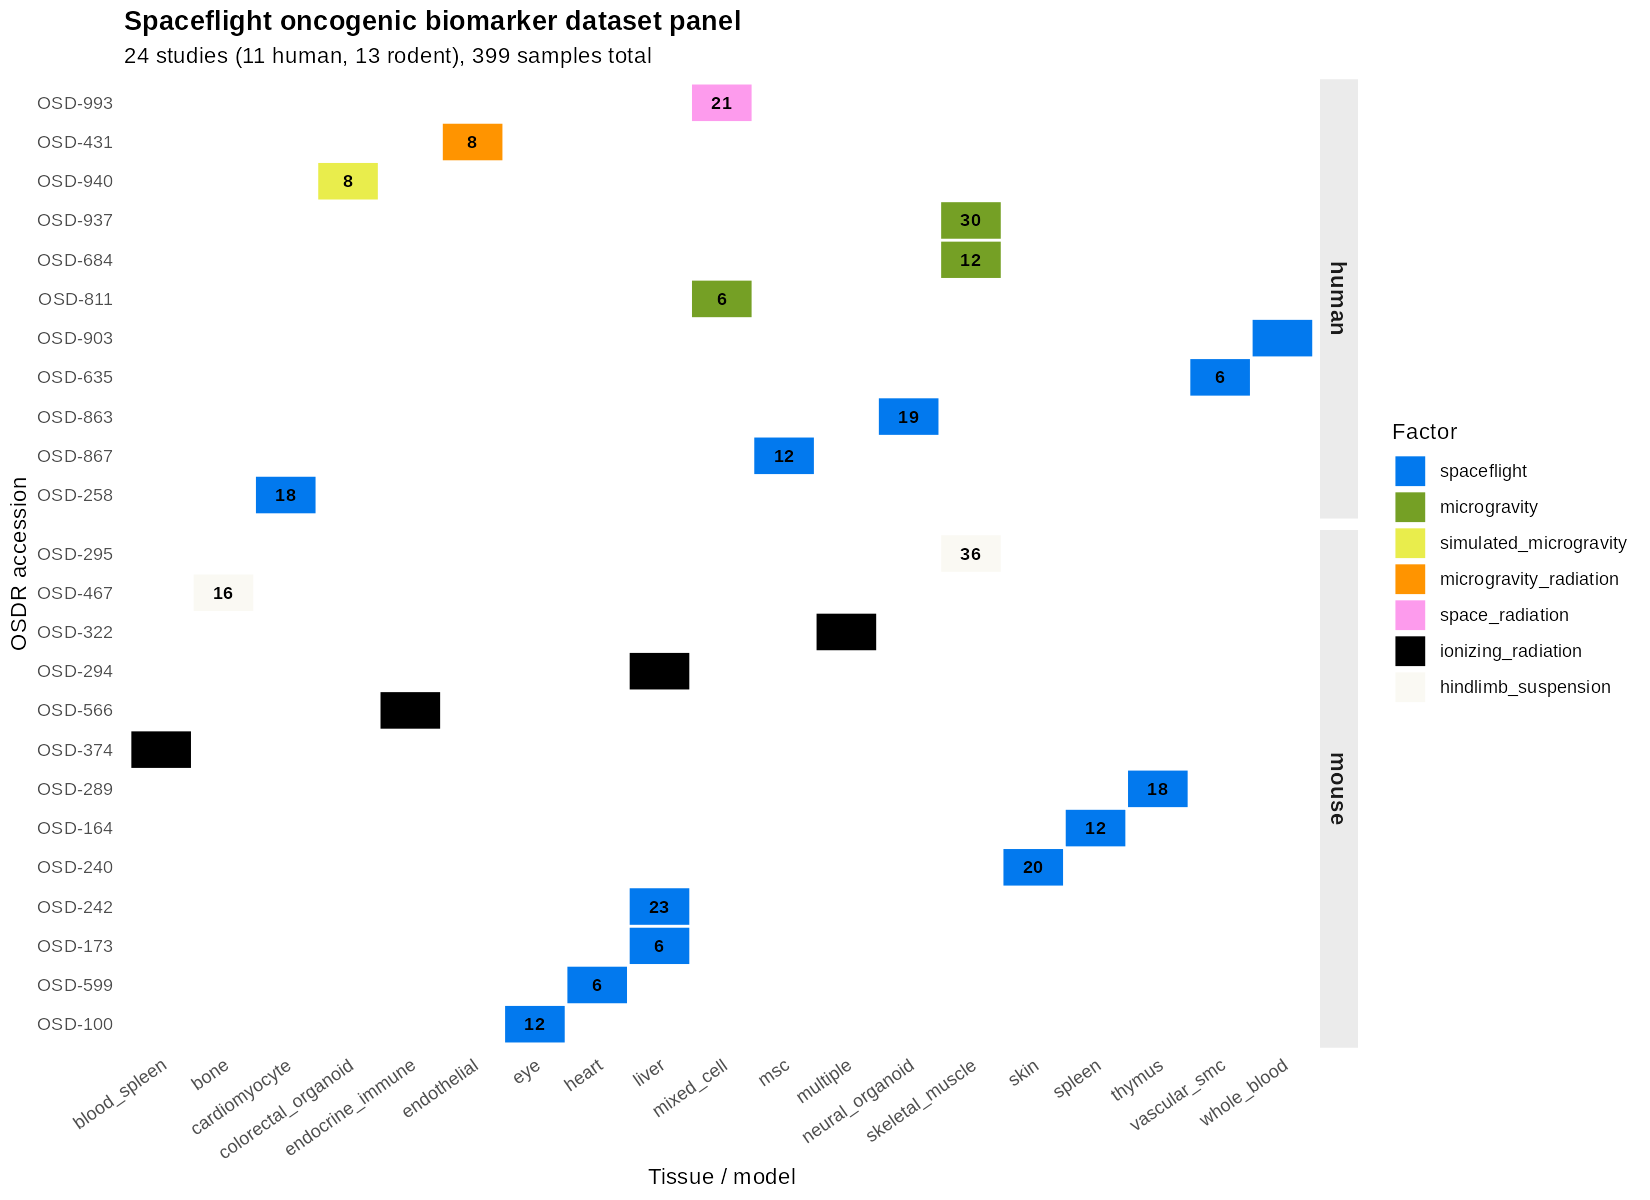
\includegraphics[width=\textwidth]{F1_dataset_panel_overview.png}
\caption{\textbf{Dataset panel overview.} The curated panel of spaceflight RNA-seq
studies (human and rodent) by tissue, stressor, and species.}
\label{fig:f1}
\end{figure}

\begin{figure}[htbp]
\centering
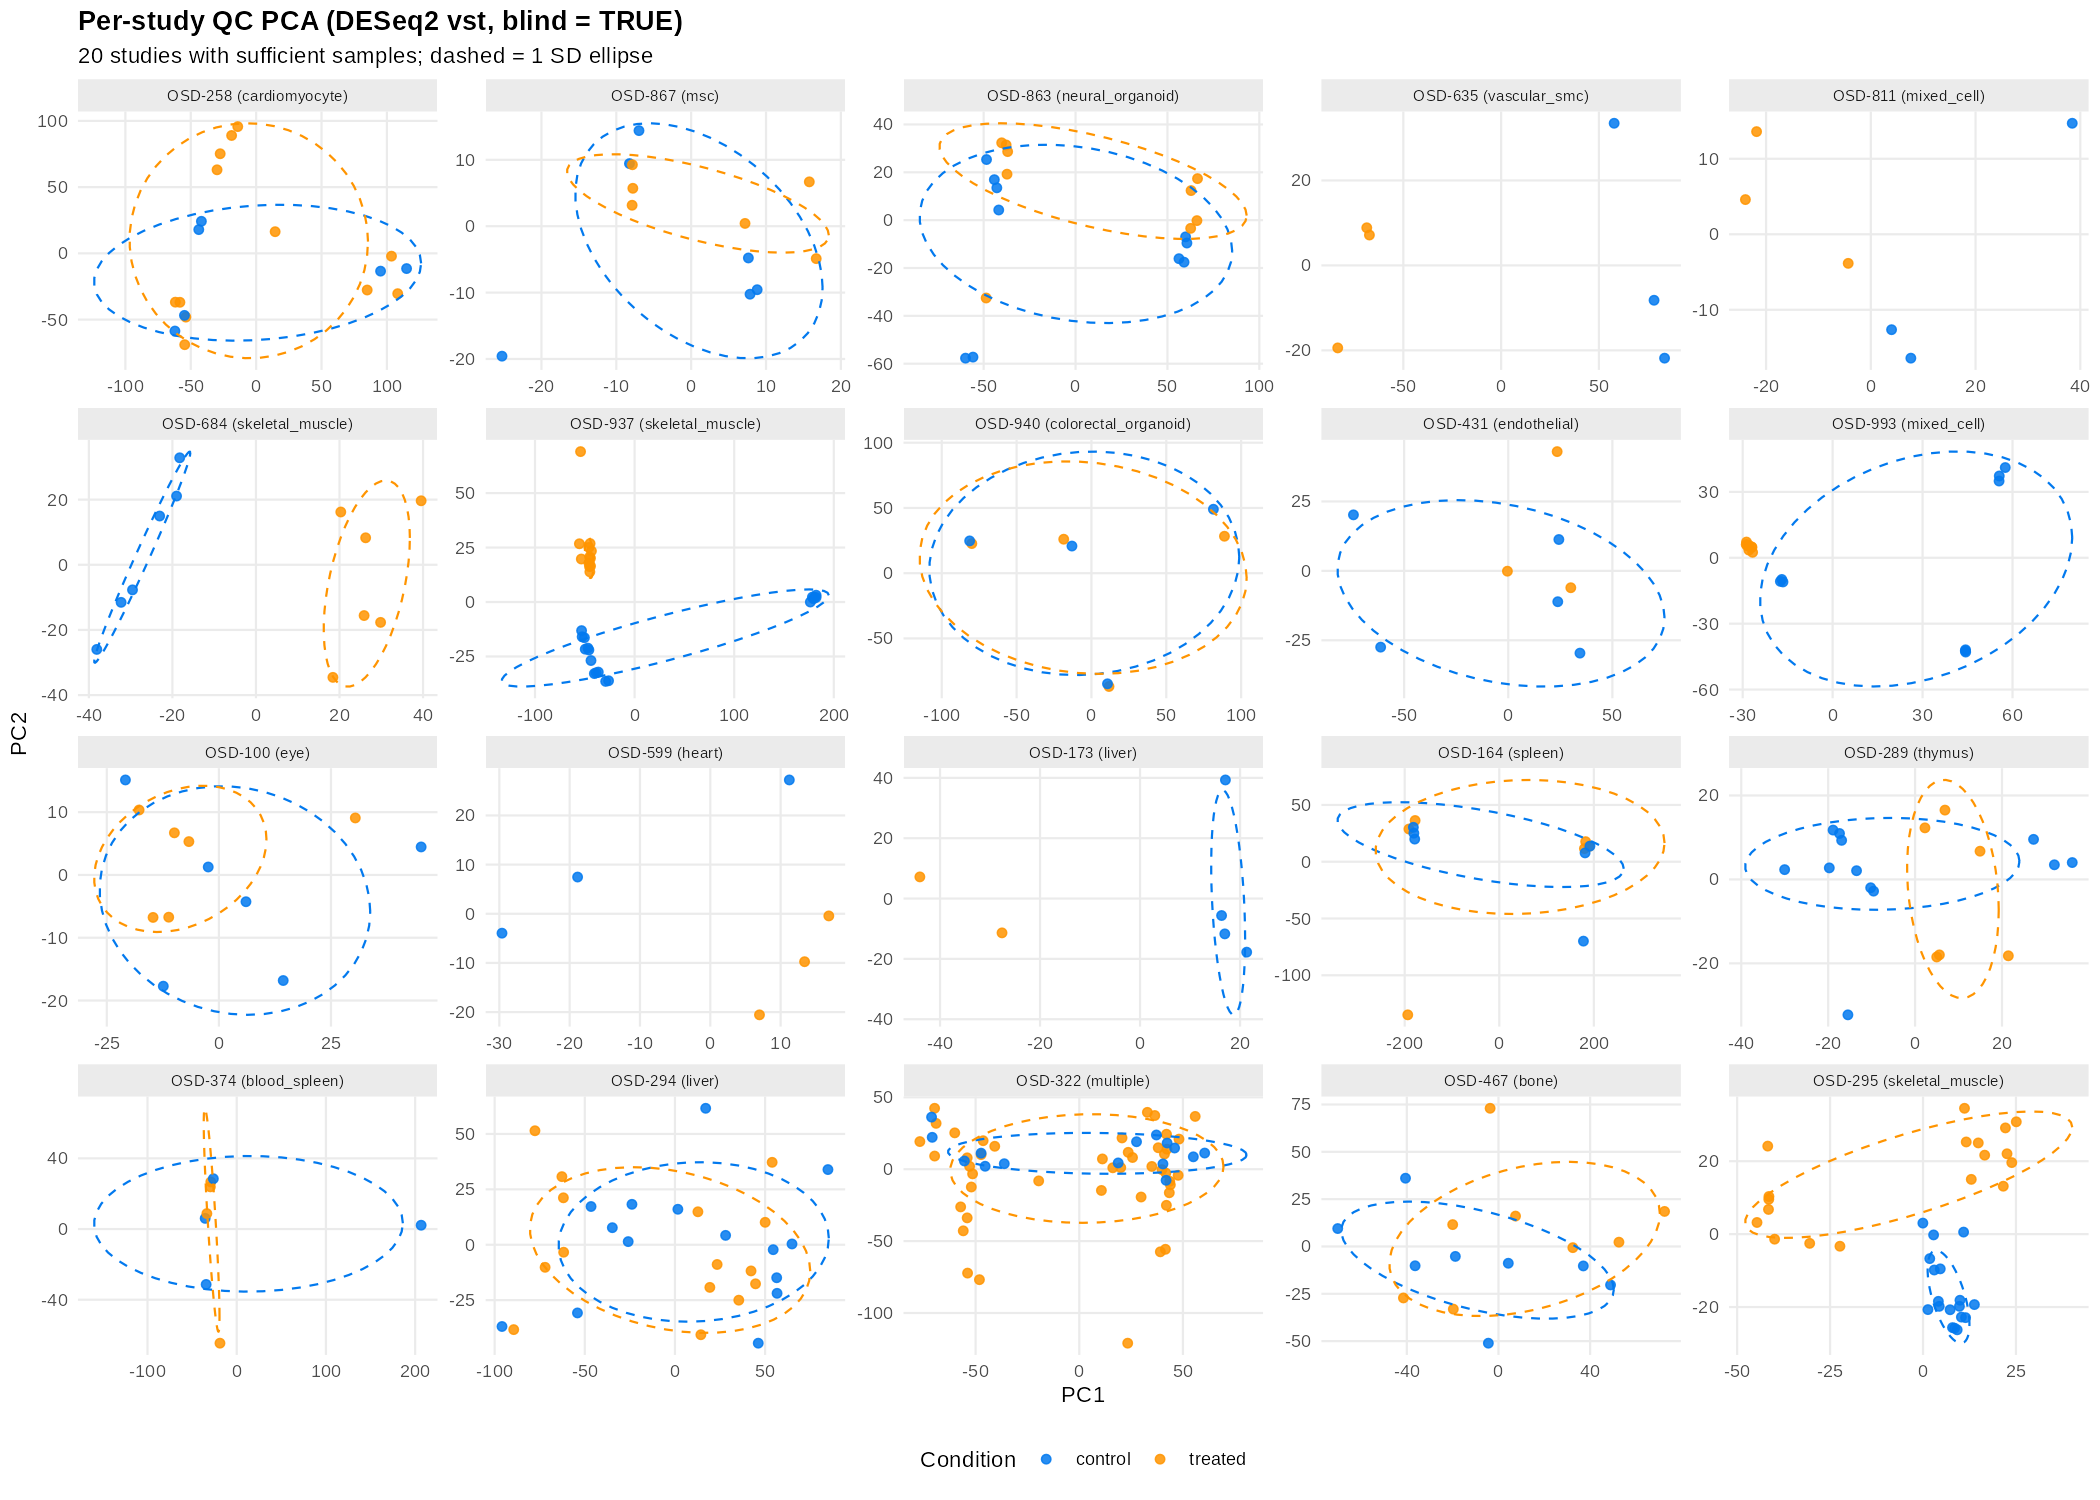
\includegraphics[width=0.85\textwidth]{F2_qc_pca.png}
\caption{\textbf{Quality control.} Principal-component analysis of per-study
expression after processing.}
\label{fig:f2}
\end{figure}

\begin{figure}[htbp]
\centering
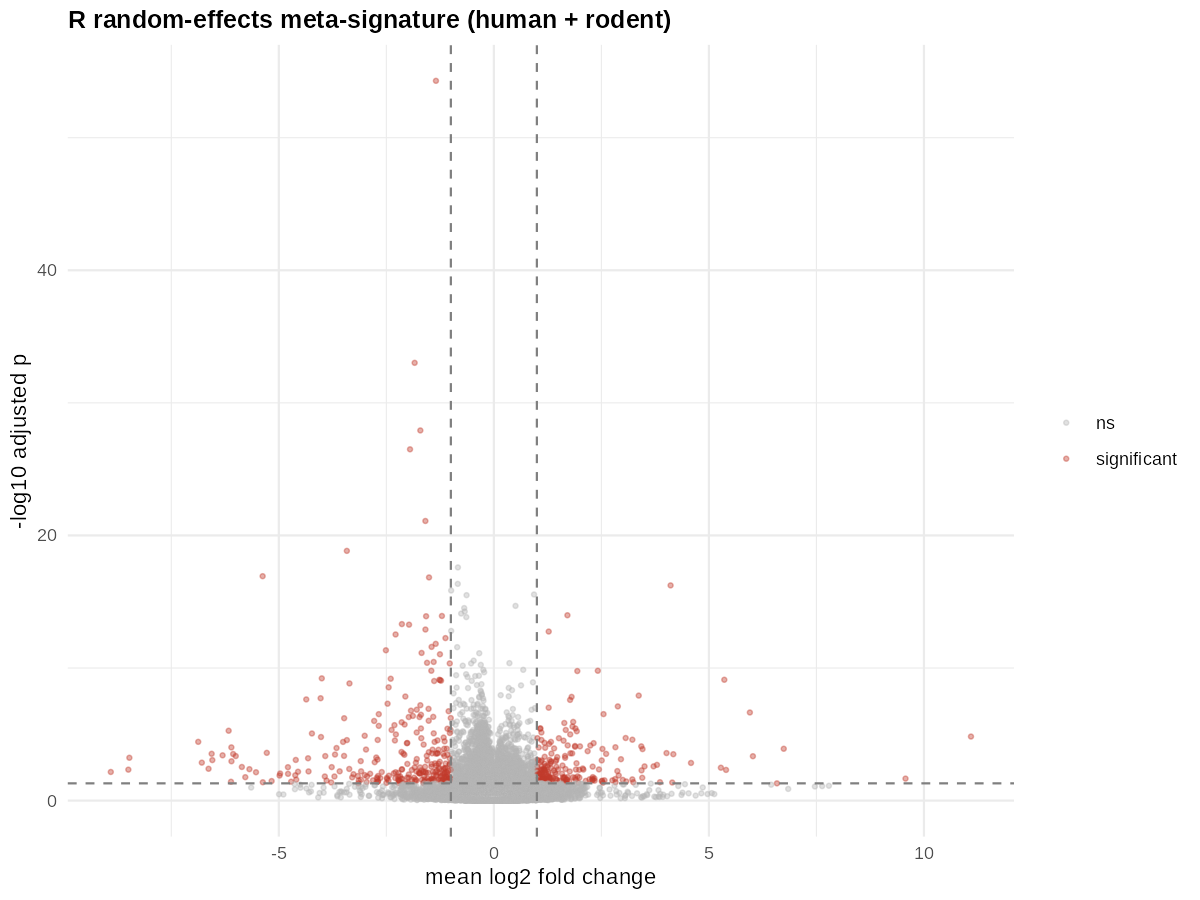
\includegraphics[width=0.85\textwidth]{F3_meta_signature_volcano.png}
\caption{\textbf{Meta-signature volcano.} Random-effects meta-analysis (metafor
REML) across 23 studies; 3{,}668 genes significant at \(p_{\mathrm{adj}} < 0.05\).}
\label{fig:f3}
\end{figure}

\begin{figure}[htbp]
\centering
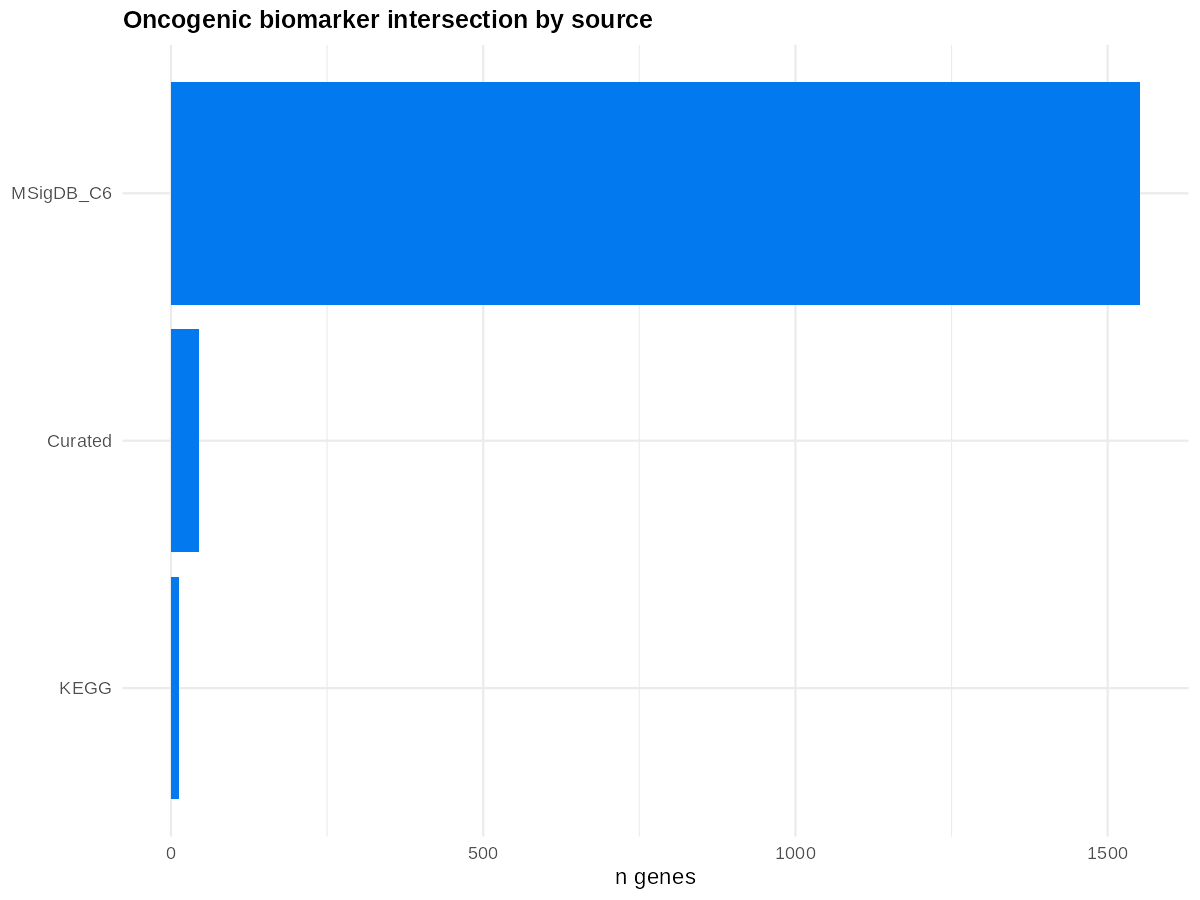
\includegraphics[width=0.48\textwidth]{F4_oncogene_intersection.png}\hfill
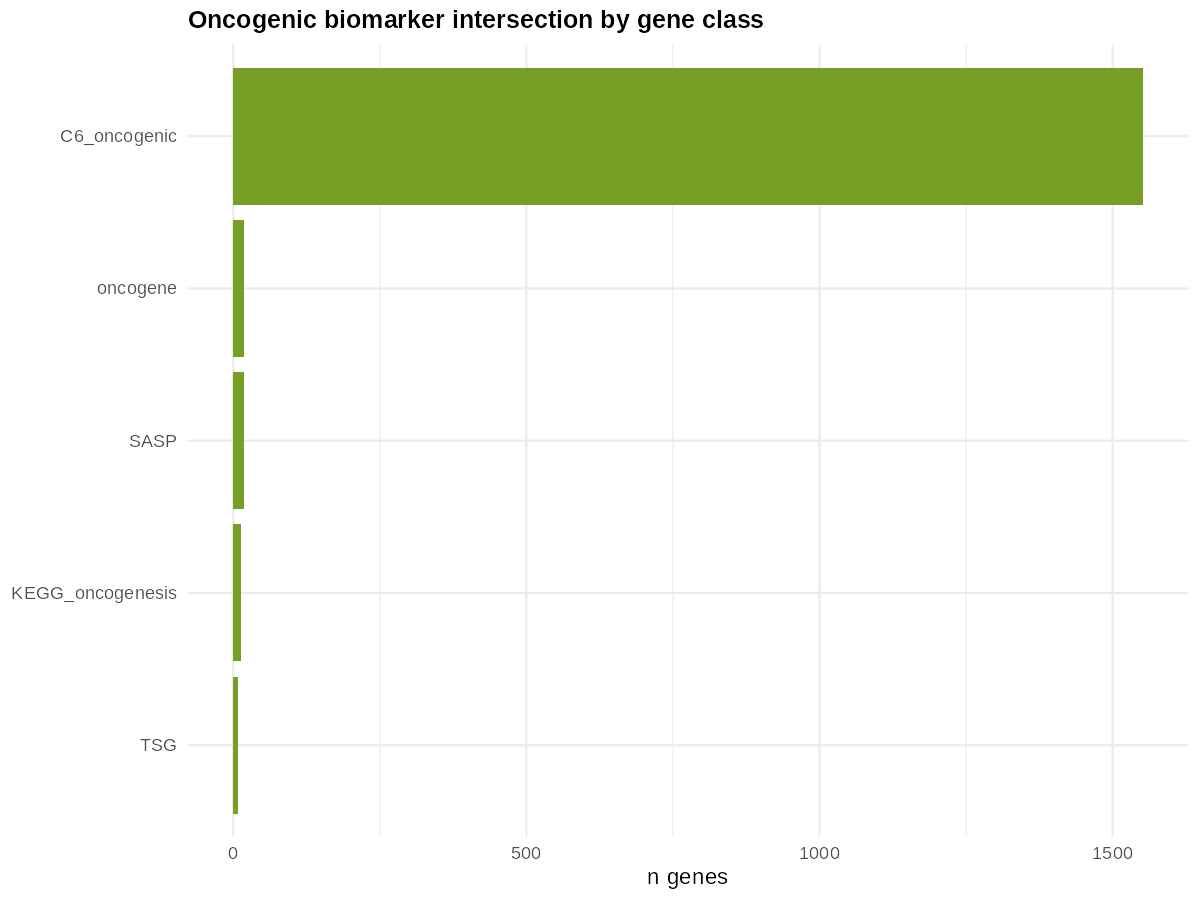
\includegraphics[width=0.48\textwidth]{F4b_oncogene_by_class.png}
\caption{\textbf{Oncogene intersection.} (a) Intersection of meta-significant genes
with the 11{,}241-gene oncogene union, yielding 1{,}610 oncogenic biomarker genes.
(b) Biomarker genes by oncogene-union class.}
\label{fig:f4}
\end{figure}

\begin{figure}[htbp]
\centering
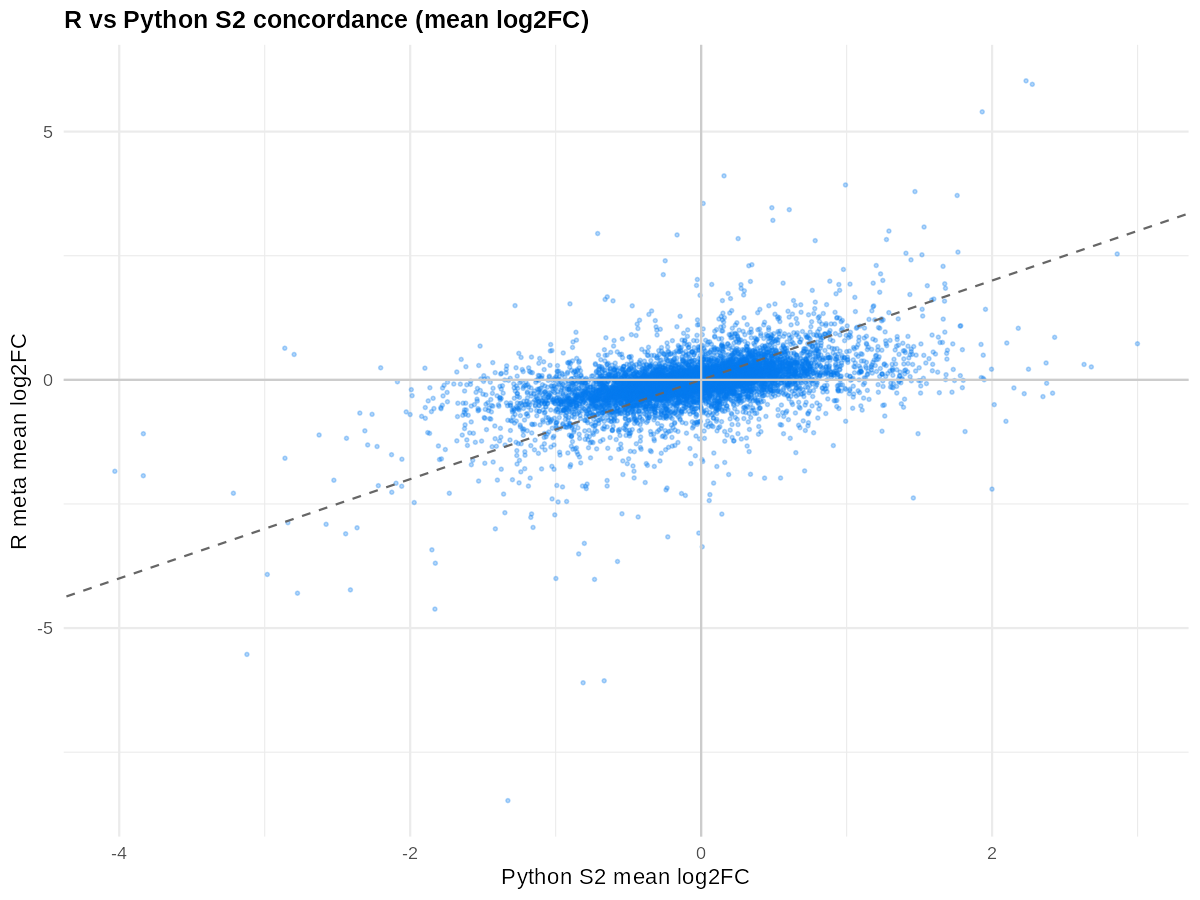
\includegraphics[width=0.75\textwidth]{F5_validation_concordance.png}
\caption{\textbf{Validation concordance.} Agreement between the R meta-signature
and an independent Python cross-study meta-signature (S2): Spearman \(\rho = 0.60\),
76\% sign agreement.}
\label{fig:f5}
\end{figure}

\subsection{Opposite-forcing drug screen identifies 21 reversal candidates}

We screened 420 LINCS L1000 GEO drug perturbation signatures (z-score profiles over
35{,}238 genes) for transcriptomic reversal of the 1{,}610 oncogenic biomarkers via
a tau-analog weighted connectivity score (WCS; \cite{lamb2006,subramanian2017}
formulation, tau-normalised across all drug signatures; Table~6). Twenty-one
compounds exhibited maximal reversal (\(\tau = -100\); Table~7, Fig.~\ref{fig:f6}),
including the food-derived flavonoids \textbf{apigenin and luteolin} (GSE128097),
\textbf{licochalcone A} (GSE137934, a licorice-derived flavonoid), the MDM2
inhibitor Nutlin-3, the topoisomerase inhibitor doxorubicin (Phase 3), PI3K-mTOR
inhibitors, a combined MEKi+WNT treatment, the DNA methylation inhibitor
5\('\)-Aza, methotrexate, the ALK5/TGF\(\beta\) inhibitor SB431542, and ketamine.

Tissue-stratified reversal scoring across 19 tissues (4{,}620 tissue-drug
combinations; Table~8, Fig.~\ref{fig:f7}) confirmed that reversal strength varies
by tissue, consistent with the tissue-specific direction of oncogenic program
engagement. Drug-target-indication context from the Broad Drug Repurposing Hub and
PrimeKG (Table~9, Fig.~\ref{fig:f9}) annotated 7 of the top 50 hits with clinical
phase, mechanism of action, and target information.

\begin{figure}[htbp]
\centering
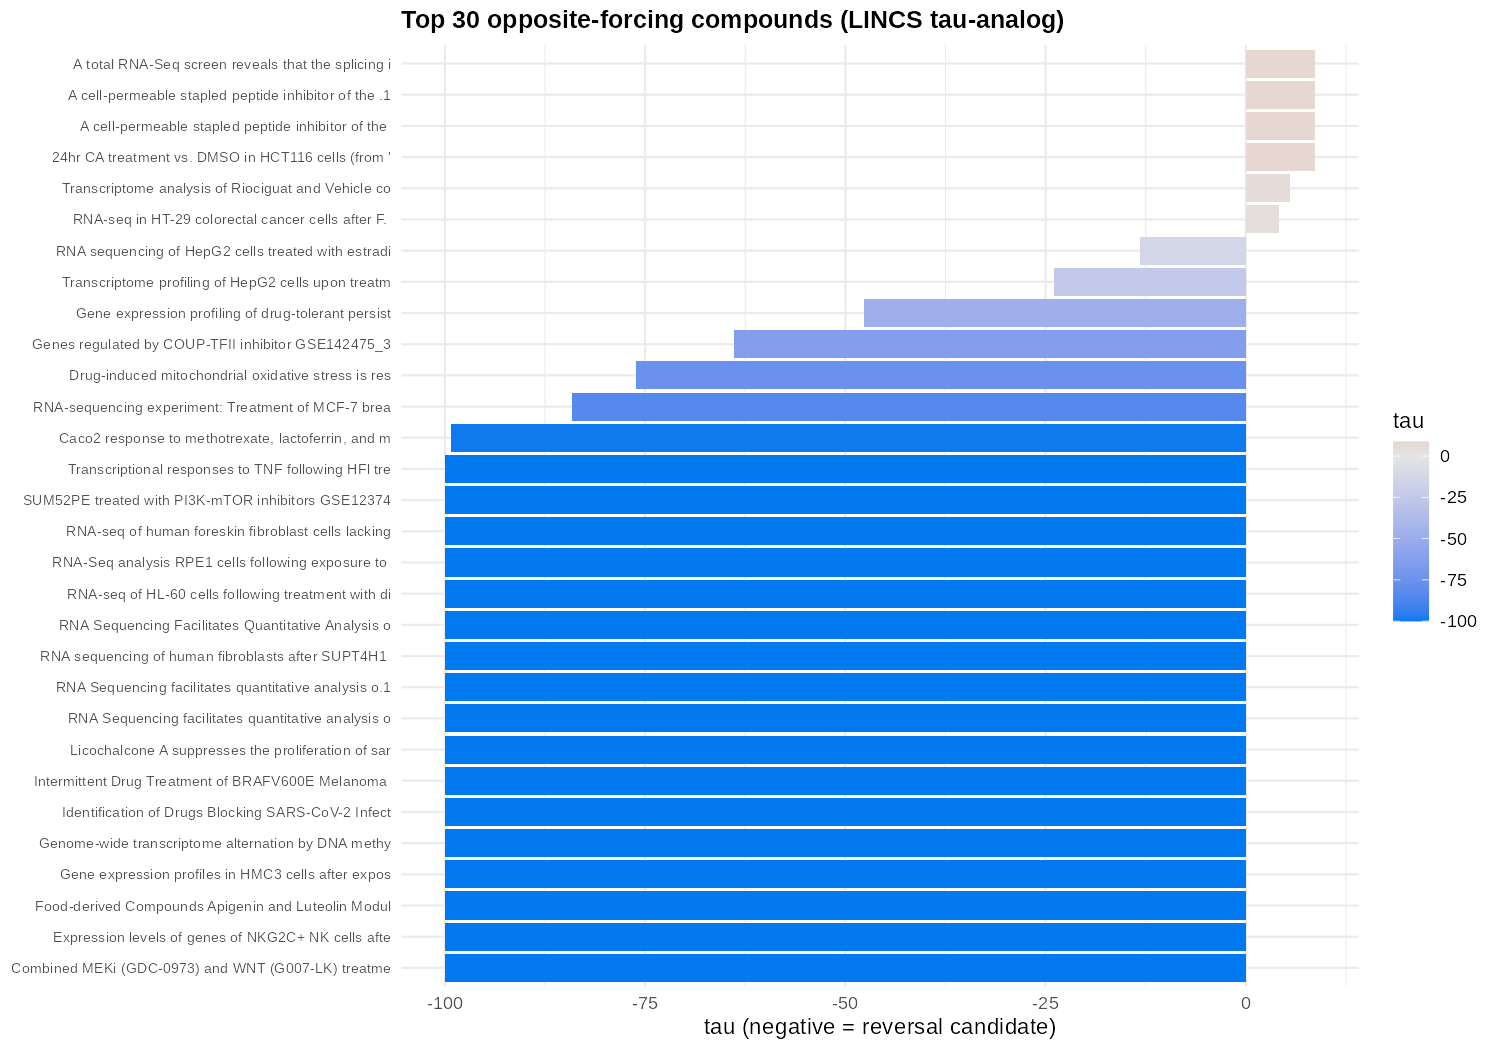
\includegraphics[width=0.85\textwidth]{F6_lincs_reversal_ranking.png}
\caption{\textbf{LINCS reversal ranking.} Tau-analog connectivity scores across 420
drug signatures; 21 compounds reach maximal reversal (\(\tau = -100\)).}
\label{fig:f6}
\end{figure}

\begin{figure}[htbp]
\centering
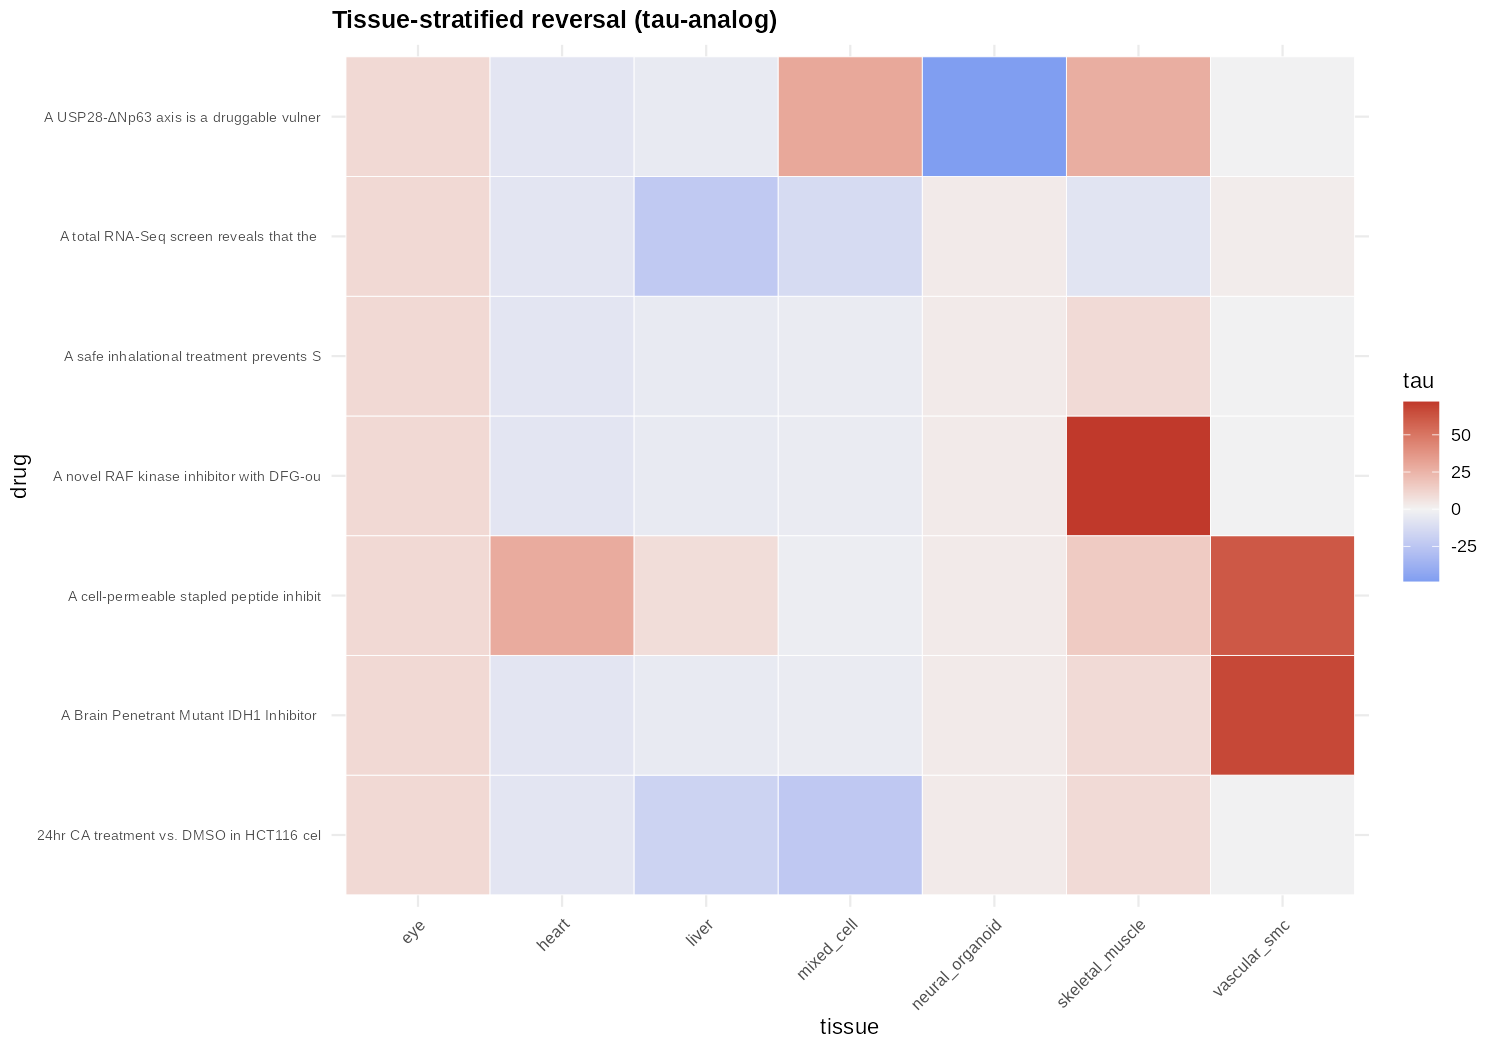
\includegraphics[width=0.85\textwidth]{F7_tissue_stratified_reversal.png}
\caption{\textbf{Tissue-stratified reversal.} Reversal strength across 19 tissues
(4{,}620 tissue-drug combinations).}
\label{fig:f7}
\end{figure}

\subsection{Gene-level reversal by food-derived flavonoids}

Because apigenin, luteolin, and licochalcone A were among the strongest reversal
candidates and are dietary compounds relevant to the ``vegan astronaut'' nutrition
goal, we examined which of the 1{,}610 oncogenic biomarker genes they directly
reverse at the gene level. We extracted the LINCS z-score vectors for the three
flavonoid signatures --- GSE128097\_1 (apigenin + luteolin co-treatment, \(\tau =
-100\)), GSE128097\_2 (apigenin + luteolin second sub-signature, \(\tau = +8.7\)),
and GSE137934\_1 (licochalcone A, \(\tau = -100\)) --- and compared each gene's
compound z-score direction against its spaceflight meta-log2FC direction.

Of the 1{,}610 oncogenic biomarker genes, 1{,}540 (95.7\%) were present in the
LINCS gene space; the remaining 70 (non-protein-coding or unmapped identifiers)
were excluded. A gene was defined as ``directly reversed'' when its spaceflight
direction (sign of mean log2FC) was opposite to its compound z-score direction,
with \(|z| \geq 1.5\) (a moderate LINCS effect threshold; sensitivity analyses at
\(|z| \geq 2\) and \(|z| \geq 3\) are reported).

\textbf{242 unique oncogenic biomarker genes (15.7\% of the 1{,}540 assessable)
were directly reversed by at least one flavonoid signature at \(|z| \geq 1.5\)}
(Table~13c, Fig.~\ref{fig:f11}). Of these, 20 were reversed by all three
signatures, 87 by two, and 135 by one. Per-signature reversal counts were:
apigenin+luteolin\_1: 134 reversed (ratio 0.55); apigenin+luteolin\_2: 136 reversed
(ratio 0.52); licochalcone A: 99 reversed (ratio 0.49) (Table~13b). At the stricter
\(|z| \geq 2\) threshold, 148 genes were reversed; at \(|z| \geq 3\), 67 genes. The
reversal ratio increased with threshold (0.49--0.55 at \(|z| \geq 1.5\) to
0.60--0.70 at \(|z| \geq 3\)), indicating that stronger compound effects are
enriched for reversal over concordance.

The most strongly reversed genes (ranked by reversal score \(= -\operatorname{sign}
(\text{mean\_lfc}) \times z \times |\text{mean\_lfc}|\); Table~13c,
Fig.~\ref{fig:f12}) were dominated by inflammatory chemokines and
senescence-associated secretory phenotype (SASP) factors that spaceflight
down-regulates and flavonoids up-regulate: \textbf{CXCL8} (interleukin-8, \(z =
8.49\), reversed by 2 signatures), \textbf{MMP3} (\(z = 4.92\), reversed by all 3),
\textbf{CSF2} (GM-CSF, \(z = 6.13\), all 3), \textbf{CSF3} (G-CSF, \(z = 3.82\)),
\textbf{CXCL3} (\(z = 4.88\), all 3), \textbf{AREG} (amphiregulin, \(z = 6.80\), all
3), and \textbf{HAS1} (\(z = 3.98\)). Genes up-regulated by spaceflight and
down-regulated by flavonoids included \textbf{DMRT1} (\(z = -4.03\)) and
\textbf{REN} (renin, \(z = -6.42\), reversed by licochalcone A). The class
distribution of reversed genes was 224 C6 oncogenic, 11 SASP, 5 oncogene, 1
tumour suppressor, and 1 KEGG oncogenesis.

Notably, GSE128097\_2 --- whose signature-level tau was \(+8.7\) (not a reversal at
the WCS level) --- still reversed 136 individual genes at \(|z| \geq 1.5\),
demonstrating that a signature that does not globally reverse a disease profile can
still counter-regulate a substantial subset of individual biomarker genes. This
underscores the value of gene-level analysis beyond signature-level connectivity
scoring.

\begin{figure}[htbp]
\centering
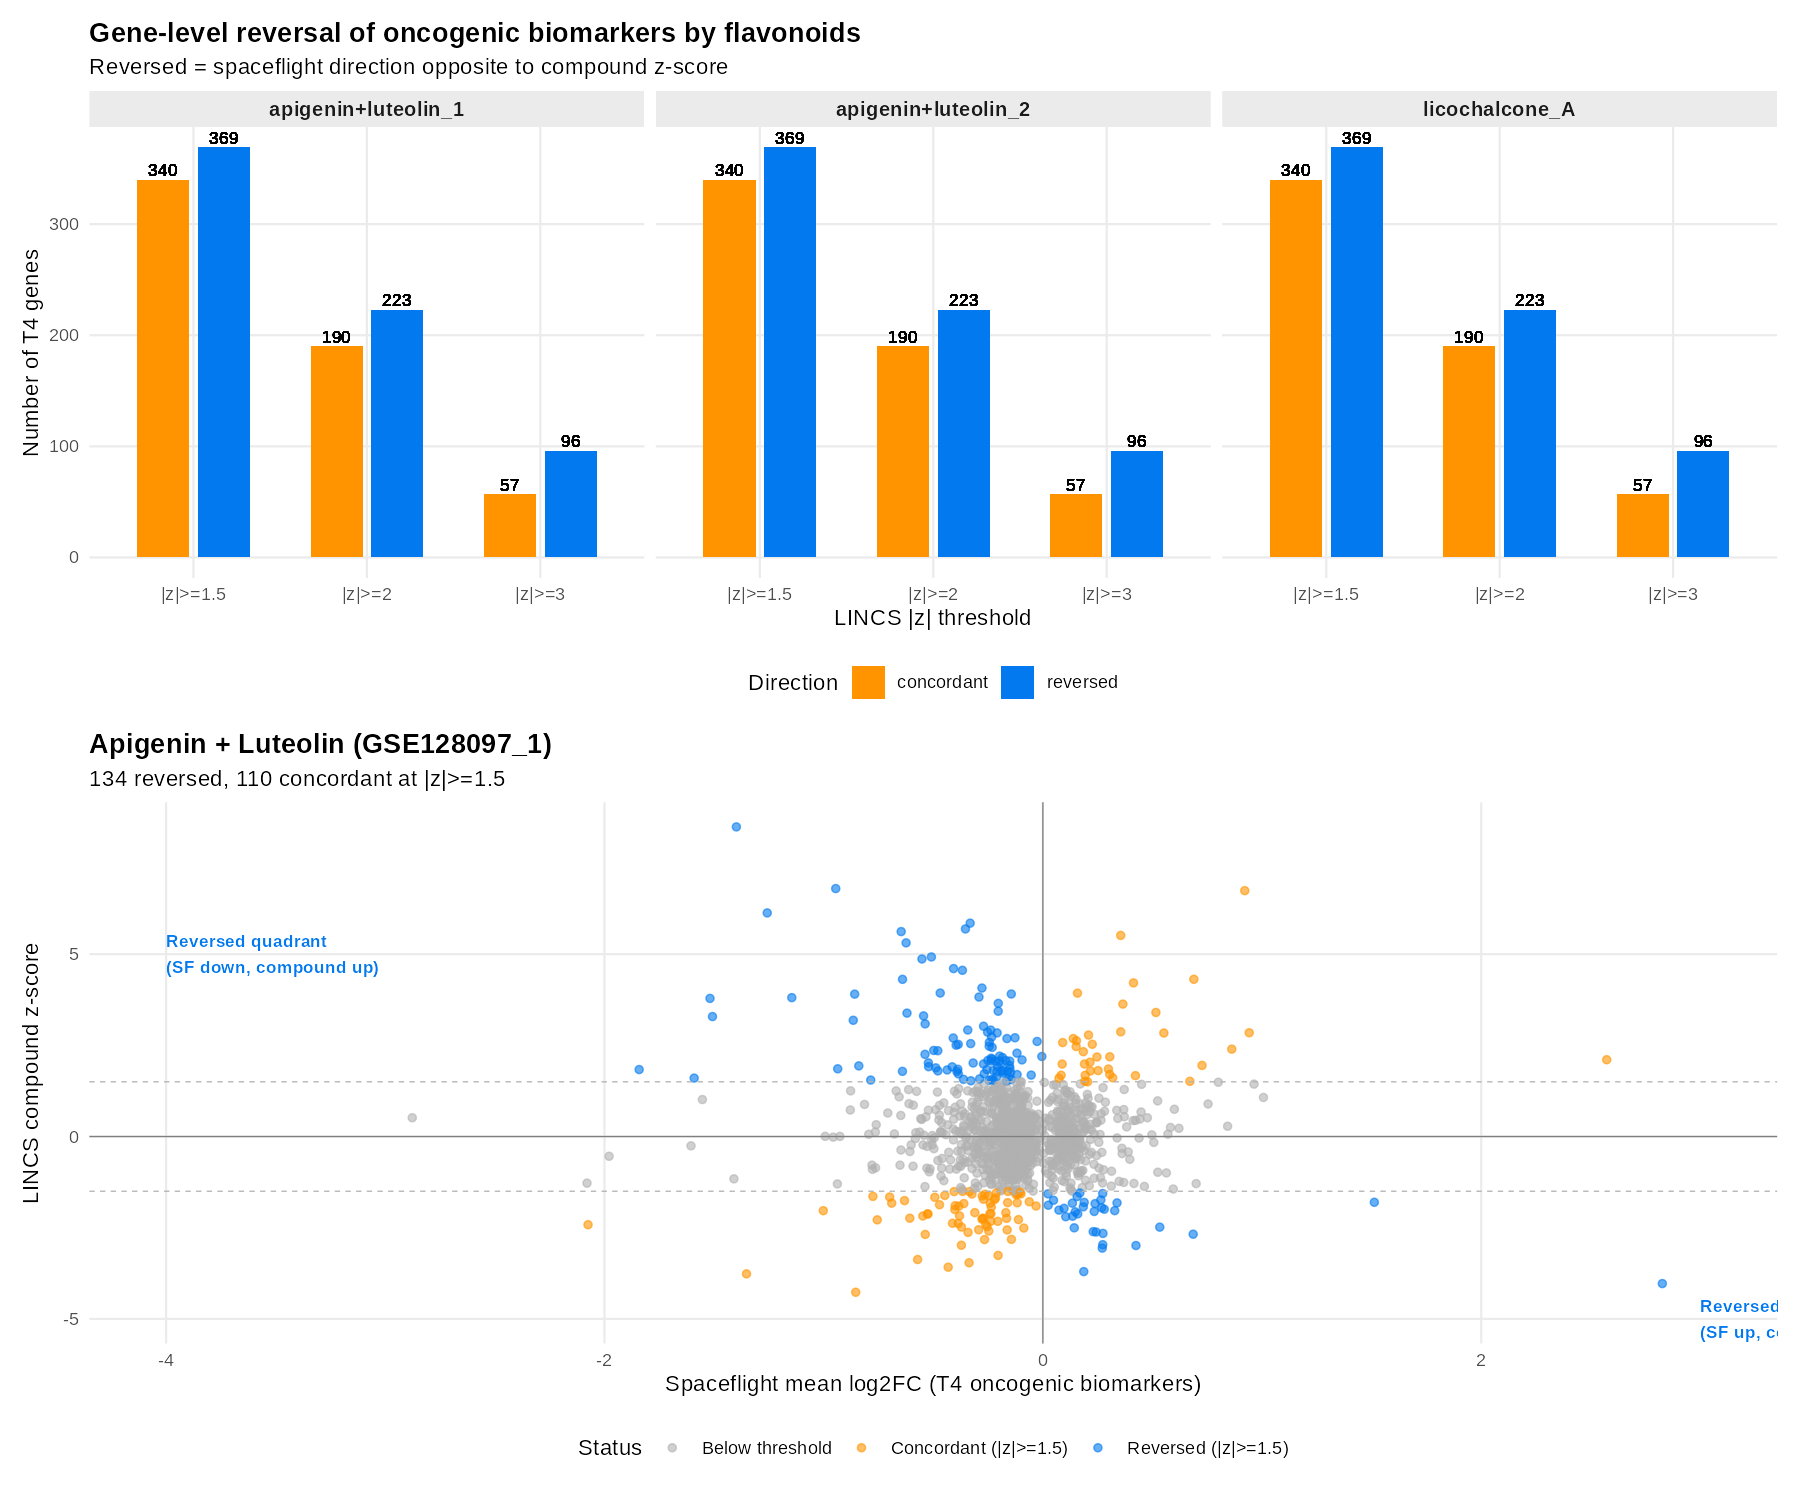
\includegraphics[width=0.85\textwidth]{F11_gene_level_reversal.png}
\caption{\textbf{Gene-level reversal.} Oncogenic biomarker genes directly reversed
by the three flavonoid signatures (\(|z| \geq 1.5\)); 242 genes reversed by at
least one.}
\label{fig:f11}
\end{figure}

\begin{figure}[htbp]
\centering
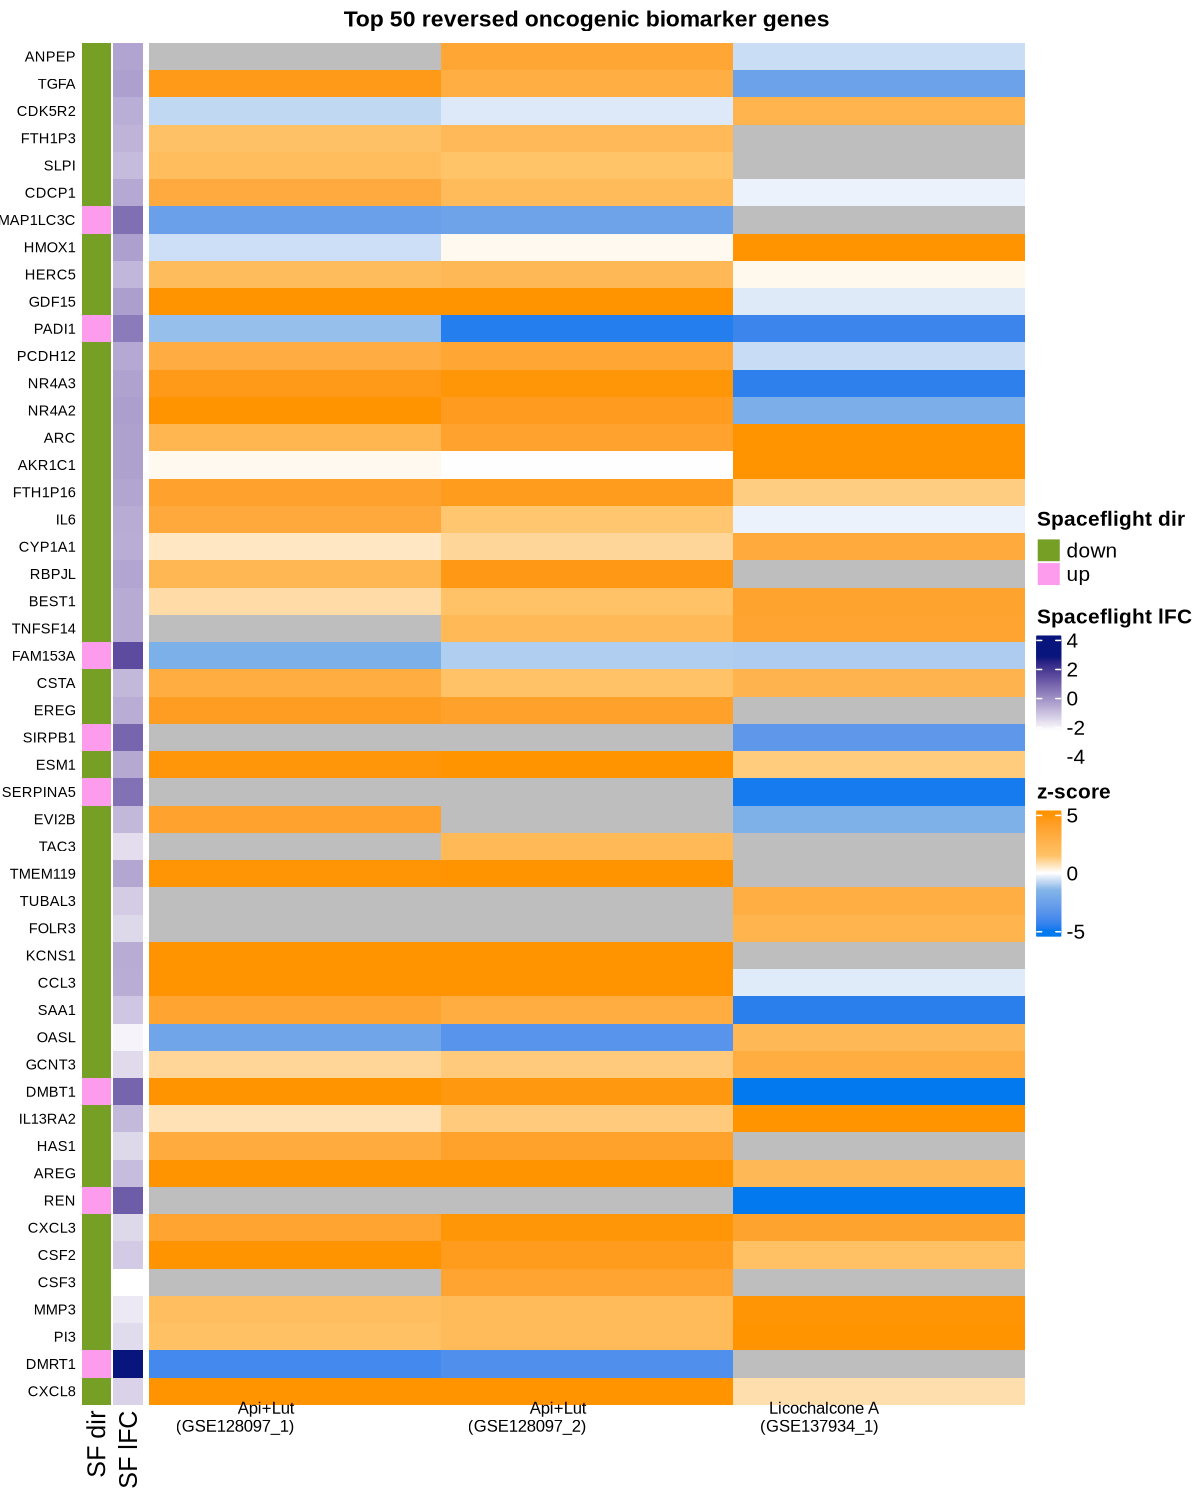
\includegraphics[width=0.85\textwidth]{F12_reversed_genes_heatmap.png}
\caption{\textbf{Reversed-gene heatmap.} Top reversed oncogenic biomarker genes,
showing spaceflight meta-log2FC versus flavonoid compound z-scores.}
\label{fig:f12}
\end{figure}

\subsection{Disease enrichment of the oncogenic biomarker signature}

To validate that the 1{,}610 oncogenic biomarker genes are biologically linked to
disease phenotypes rather than noise, we performed hypergeometric enrichment
against PrimeKG (160{,}822 disease-gene edges) \cite{chandrasekharan2023} and
gene-disease association scoring via the Open Targets GraphQL API \cite{ochoa2023}.

PrimeKG yielded 389 significant diseases (\(p_{\mathrm{adj}} < 0.05\); Table~10),
led by sarcomatoid carcinoma (\(p_{\mathrm{adj}} = 3.3 \times 10^{-12}\), 47
overlapping genes), undifferentiated carcinoma (\(3.3 \times 10^{-12}\)), coronary
artery disease (\(3.4 \times 10^{-11}\), 58 genes), carcinoma (\(4.5 \times
10^{-11}\)), and prostate cancer. Open Targets returned 4{,}891 gene-disease
associations for 100 queried genes across 1{,}689 diseases (Table~11), led by
neoplasm, cancer, hepatocellular carcinoma, breast carcinoma, breast cancer, NSCLC,
Alzheimer's disease, glioblastoma, melanoma, and colorectal carcinoma. A
cross-ranked combined table (Table~10b, Fig.~\ref{fig:f8}) integrated both sources,
with breast carcinoma, breast cancer, hepatocellular carcinoma, and prostate
carcinoma ranking highest by combined score.

\begin{figure}[htbp]
\centering
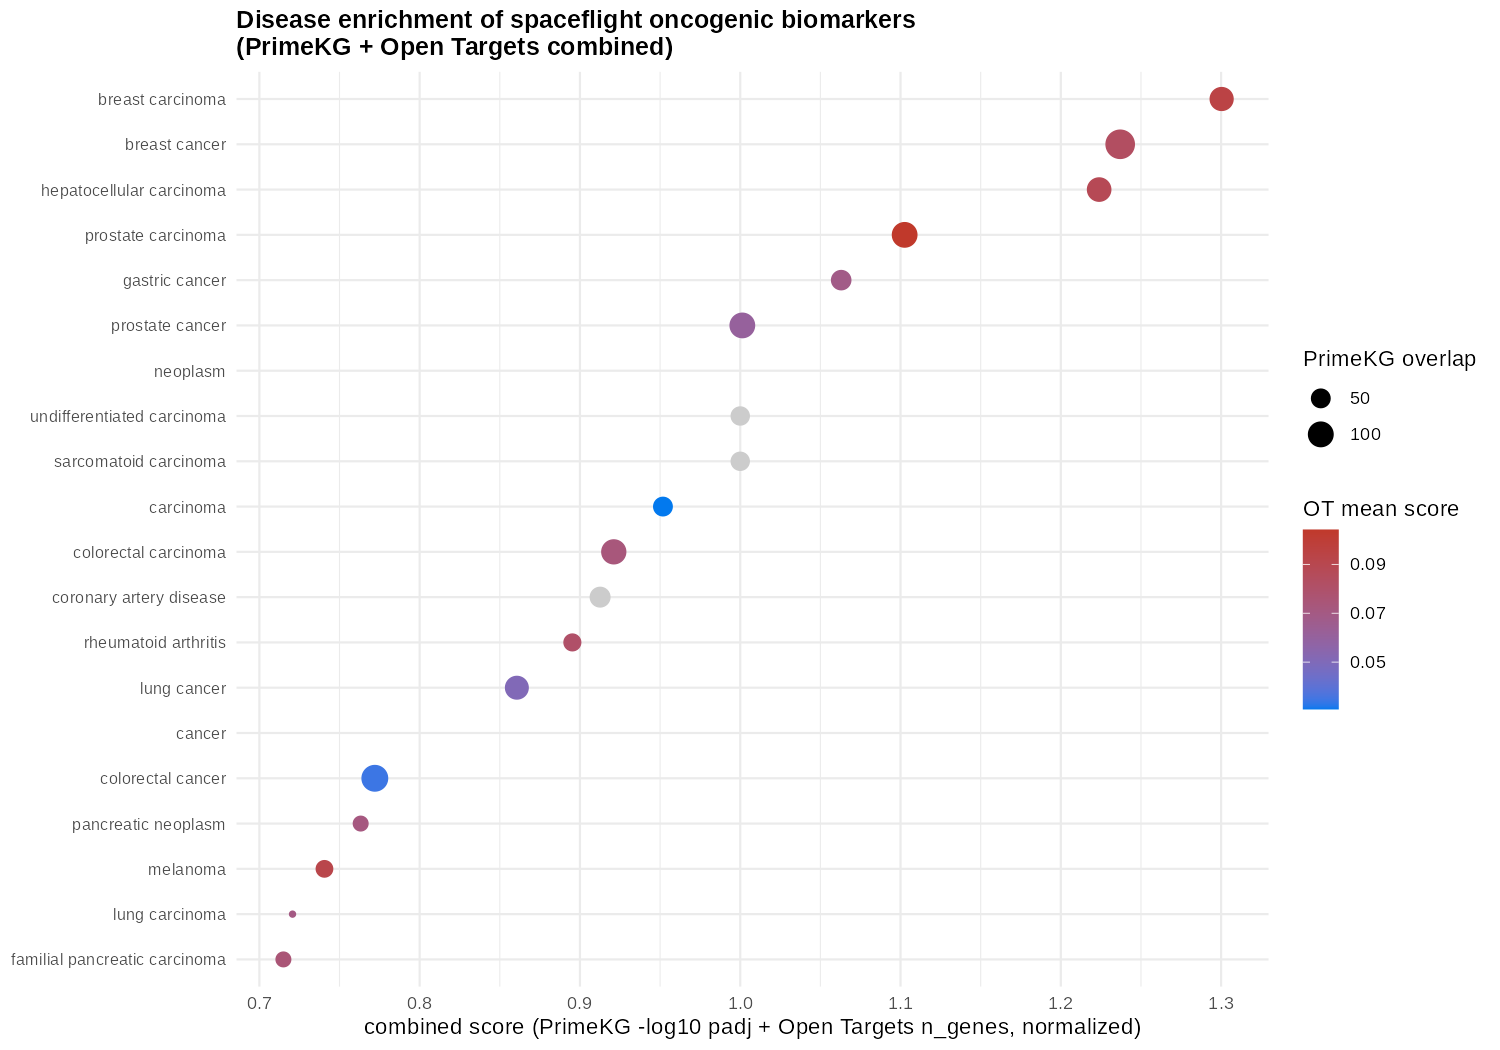
\includegraphics[width=0.85\textwidth]{F8_disease_enrichment.png}
\caption{\textbf{Disease enrichment.} Combined PrimeKG hypergeometric enrichment and
Open Targets gene-disease association ranking for the 1{,}610 biomarker genes.}
\label{fig:f8}
\end{figure}

\begin{figure}[htbp]
\centering
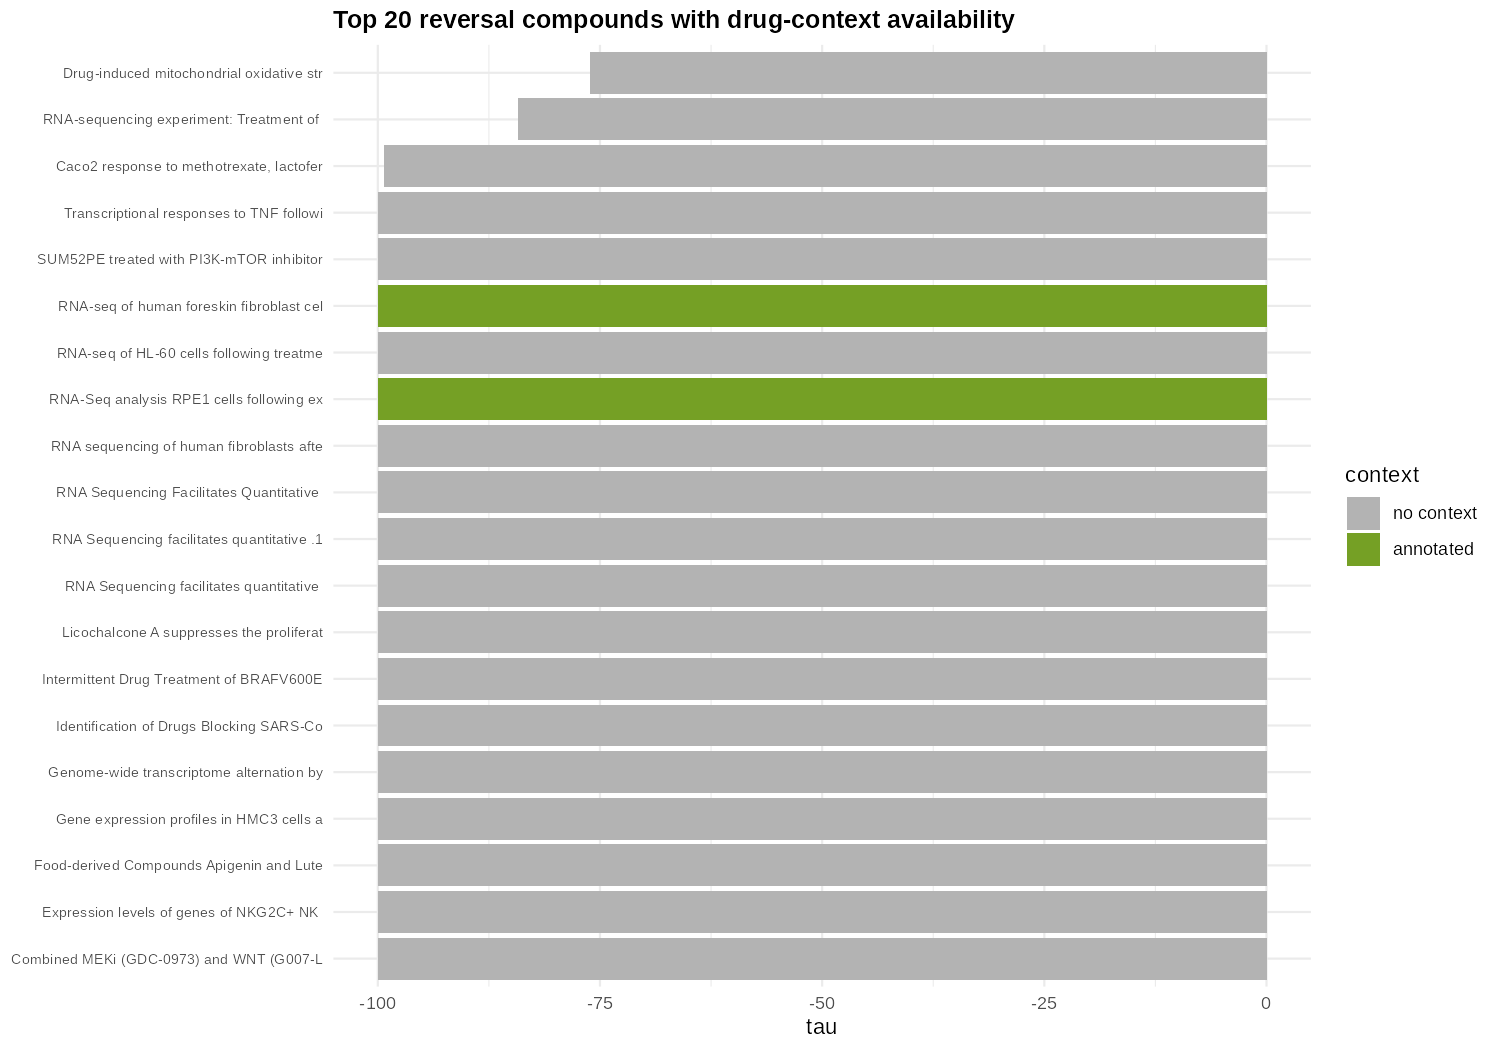
\includegraphics[width=0.85\textwidth]{F9_drug_context.png}
\caption{\textbf{Drug context.} Clinical phase, mechanism of action, target, and
indication annotation of top reversal hits (Broad Drug Repurposing Hub, PrimeKG).}
\label{fig:f9}
\end{figure}

\subsection{Nutraceutical candidates among reversal hits}

Among the top 50 reversal hits, we flagged nutraceuticals using a curated
176-compound lexicon (17 classes: flavonoids, stilbenes, curcuminoids, carotenoids,
vitamins, glucosinolates, omega-3 lipids, and others) cross-matched against LINCS
GMT drug names and the Broad Drug Repurposing Hub (Table~12, Fig.~\ref{fig:f10}).
Five unique nutraceuticals were flagged: \textbf{luteolin} (\(\tau = -100\), 3
evidence streams: signature + LINCS GMT + Broad), \textbf{apigenin} (\(\tau =
-100\), 2 streams), \textbf{licochalcone A} (\(\tau = -100\), 2 streams),
licochalcone, and isoginkgetin (\(\tau = +8.7\), not a reversal --- same direction
as spaceflight). A full scan of all 420 scored signatures identified 37
nutraceutical-bearing signatures (Table~12c) as input for a deferred vegan-recipe
optimisation step.

\begin{figure}[htbp]
\centering
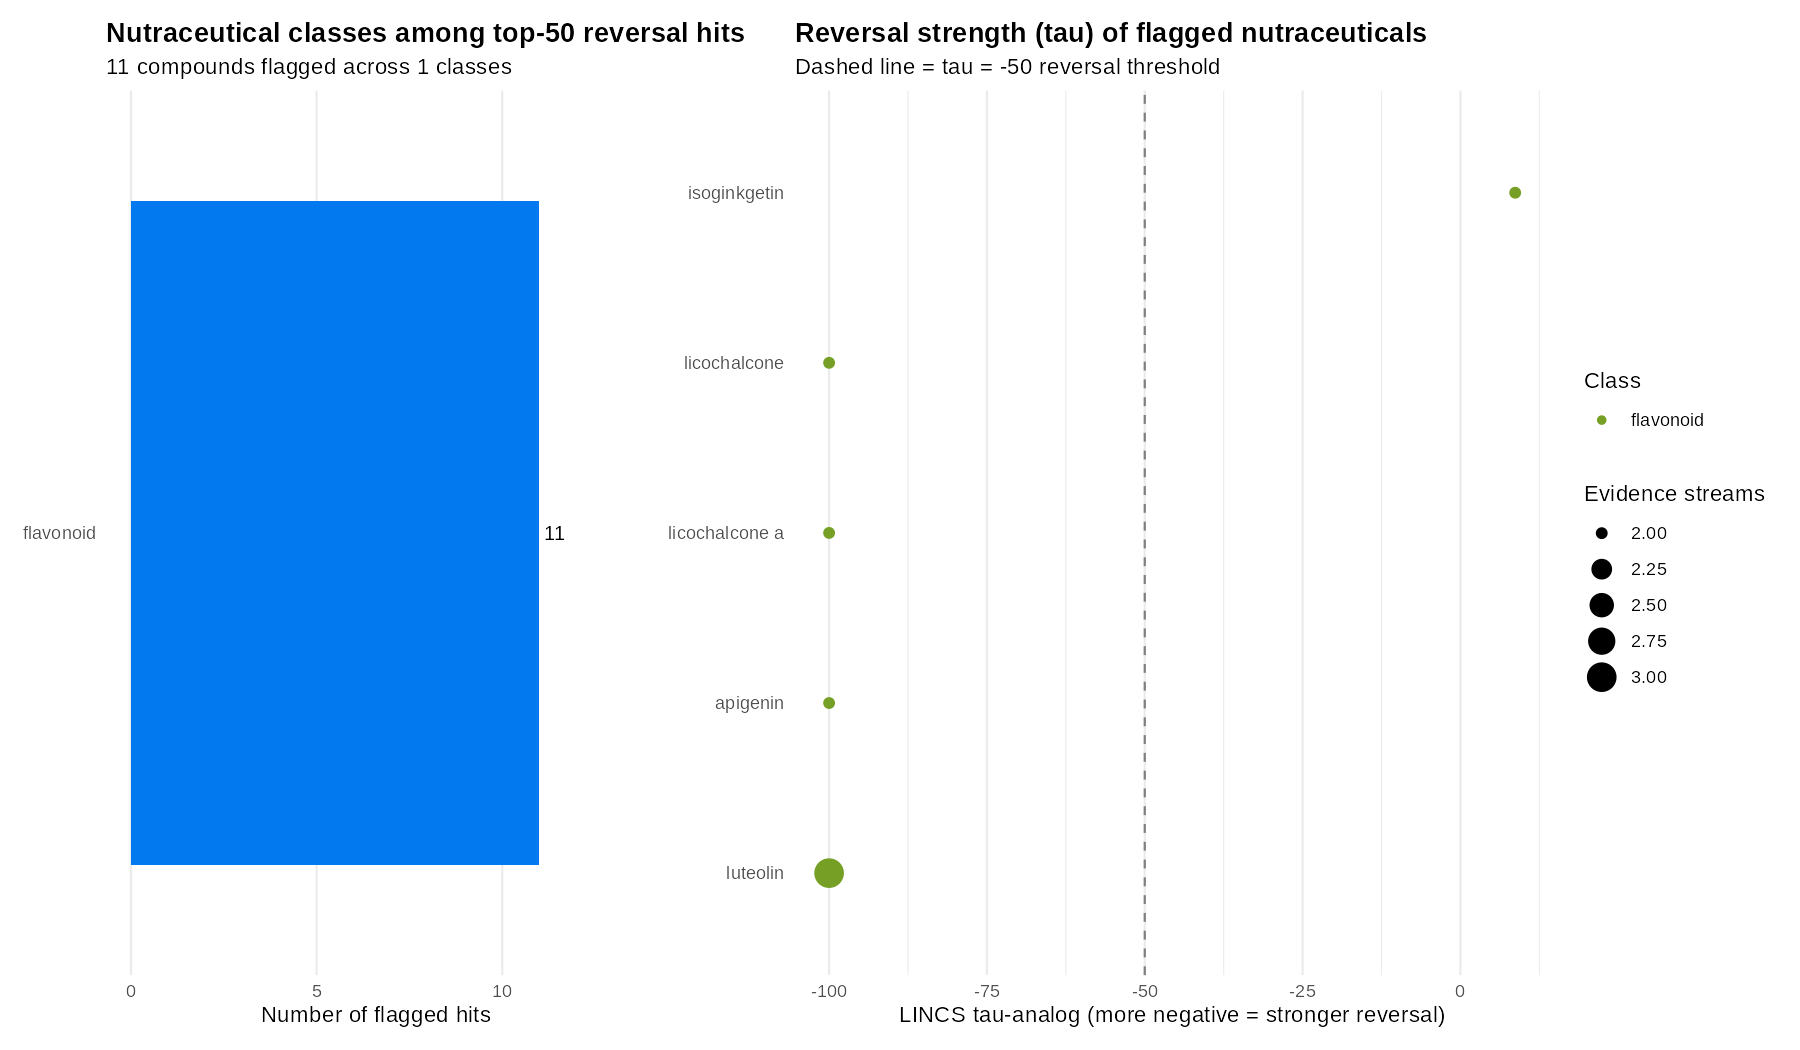
\includegraphics[width=0.85\textwidth]{F10_nutraceutical_flags.png}
\caption{\textbf{Nutraceutical flags.} Nutraceuticals among the top reversal hits,
with supporting evidence streams.}
\label{fig:f10}
\end{figure}

\section{Discussion}\label{sec:discussion}

Across a cross-species panel of 23 spaceflight RNA-seq studies, we re-derived a
1{,}610-gene oncogenic biomarker signature that concords with an independent Python
meta-analysis (Spearman \(\rho = 0.60\)) and enriches for carcinoma, coronary
artery disease, and hereditary cancer syndromes. Screening LINCS L1000 drug
perturbation signatures identified 21 compounds with maximal transcriptomic
reversal (\(\tau = -100\)), led by food-derived flavonoids. Gene-level analysis
revealed that 242 oncogenic biomarker genes (15.7\% of assessable) are directly
reversed by at least one flavonoid signature, with inflammatory chemokines and SASP
factors (CXCL8, MMP3, CSF2, CSF3, CXCL3) most strongly counter-regulated.

The convergence of flavonoid reversal on inflammatory and SASP chemokines is
biologically coherent. Spaceflight has been shown to dysregulate immune signalling
and promote a senescence-associated secretory phenotype; flavonoids such as
apigenin and luteolin are known modulators of NF-\(\kappa\)B and inflammatory
cytokine production. The finding that these dietary compounds reverse the
spaceflight-driven suppression of CXCL8, CSF2, and MMP3 at the transcriptomic level
nominates them as candidate nutritional countermeasures for prospective validation.

The gene-level analysis also revealed that signature-level and gene-level reversal
can diverge: GSE128097\_2 was not a reversal candidate at the WCS/tau level (\(\tau
= +8.7\)) yet reversed 136 individual biomarker genes. This has a practical
implication: signature-level connectivity scoring may miss compounds that reverse a
biologically important subset of a disease signature even when the global profile is
not anti-correlated. Gene-level reversal analysis should complement, not replace,
signature-level screening.

\bmhead{Limitations}
(1) The LINCS tau-analog is computed from GEO-derived z-score signatures, not the
canonical CLUE.io Touchstone GCTx with pre-computed tau; WCS values are near-zero
for most drugs, so tau-normalisation clips at \(\pm 100\). The ranking is correct
but absolute tau values are compressed. (2) GSE128097 is a co-treatment of apigenin
and luteolin; gene-level effects cannot be attributed to one compound alone. (3)
LINCS z-scores lack per-gene p-values, so the \(|z| \geq 1.5\) threshold is an
effect-size cutoff, not a statistical test; the reversal score is descriptive. (4)
COSMIC CGC and OncoKB were gated; the oncogene union relied on MSigDB C6
\cite{liberzon2015}, KEGG, and curated lists. (5) The 70 T4 genes absent from LINCS
were excluded from gene-level analysis. (6) These are transcriptomic associations,
not evidence of efficacy in vivo; the flavonoid reversal candidates require
prospective validation in spaceflight-relevant model systems. (7) Vegan recipe
optimisation is deferred; this pipeline provides the nutraceutical-gene input
(T12c, T13c) for that future step.

\section{Methods}\label{sec:methods}

\subsection{Data acquisition}
We queried the NASA OSDR API \cite{beheshti2023} for human and rodent RNA-seq
studies with processed count matrices and a testable
spaceflight/microgravity/radiation contrast, yielding 24 studies (11 human, 13
rodent; Table~1). JAXA6 astronaut whole-blood data were obtained from the
Astronaut\_health\_search GitHub repository. Raw STAR unnormalised count matrices
were downloaded per study.

\subsection{Differential expression}
Per-study DESeq2 analysis was run with the contrast
spaceflight/microgravity/radiation (treated) vs ground/vivarium/sham control. Genes
with \(p_{\mathrm{adj}} < 0.05\) and \(|\text{log2FC}| > 1\) were called
significant. Rodent gene identifiers were mapped to human orthologs via biomaRt
(getLDS with mirror retry logic; MGI symbol fallback).

\subsection{Meta-analysis}
A random-effects meta-analysis was performed per gene using \texttt{metafor::rma}
(REML, z-test) \cite{viechtbauer2010} over the per-study log2FC and standard error
values. The meta-signature comprised 40{,}211 genes with mean log2FC, standard
error, z, p, \(p_{\mathrm{adj}}\), direction concordance, and species count
(Table~3).

\subsection{Oncogene union}
We assembled an 11{,}241-gene oncogene union from MSigDB C6 oncogenic signatures
(10{,}927 genes via msigdbr) \cite{liberzon2015}, KEGG oncogenesis pathways (931 via
KEGGREST), and a curated oncogene/tumour-suppressor/SASP list (195). COSMIC CGC and
OncoKB were attempted but gated (all COSMIC URLs failed; OncoKB returned HTTP 401).
The intersection of meta-significant genes with the oncogene union yielded 1{,}610
oncogenic biomarker genes.

\subsection{LINCS tau-analog reversal screen}
We loaded the LINCS L1000 GEO z-score signature matrix (4{,}269 signatures \(\times\)
35{,}238 genes) and filtered to 420 drug-related signatures. For each drug
signature, we computed a weighted connectivity score (WCS) against the disease
UP/DN gene sets using a weighted Kolmogorov-Smirnov enrichment (CMap a-score
formulation) \cite{lamb2006,subramanian2017}, then tau-normalised across all drug
signatures (clipped to \(\pm 100\)). A strongly negative tau indicates reversal.

\subsection{Gene-level reversal}
For the three flavonoid signatures (GSE128097\_1, GSE128097\_2, GSE137934\_1), we
extracted the z-score vector over all genes and intersected with the 1{,}610
oncogenic biomarkers (1{,}540 overlap). A gene was ``directly reversed'' when
\(\operatorname{sign}(\text{spaceflight mean log2FC}) \times \operatorname{sign}
(\text{compound } z) < 0\) and \(|z| \geq 1.5\). Reversal score \(=
-\operatorname{sign}(\text{mean\_lfc}) \times z \times |\text{mean\_lfc}|\).
Sensitivity thresholds \(|z| \geq 2\) and \(|z| \geq 3\) are reported.

\subsection{Disease enrichment}
PrimeKG disease-gene edges (160{,}822) \cite{chandrasekharan2023} were tested for
hypergeometric enrichment of the 1{,}610 oncogenic biomarkers (universe = all genes
in PrimeKG disease-gene edges; BH-adjusted p-values). The Open Targets GraphQL API
(v4) \cite{ochoa2023} was queried for 100 genes, returning 4{,}891 gene-disease
associations across 1{,}689 diseases. A combined ranking integrated both sources.

\subsection{Drug context}
The Broad Drug Repurposing Hub (6{,}798 drugs; clinical phase, MoA, target,
indication) and PrimeKG drug-target (51{,}306 edges) and contraindication (61{,}350
edges) networks were used to annotate the top 50 reversal hits.

\subsection{Nutraceutical flagging}
A curated 176-compound lexicon (17 classes) was cross-matched against the top 50
reversal hits via word-boundary regex on signature names and extracted drug names,
with independent evidence from LINCS GMT drug names and the Broad Drug Repurposing
Hub.

\subsection{Software and reproducibility}
All analysis was performed in R 4.4.3 with DESeq2, limma, edgeR, biomaRt, metafor,
clusterProfiler, msigdbr, fgsea, ComplexHeatmap, KEGGREST, data.table, ggplot2, and
patchwork. Package versions are pinned in \texttt{renv.lock}. The pipeline is
executed via \texttt{run\_all.R} with \texttt{--from}/\texttt{--only} flags for
resumability. All figures are saved as SVG (editable) and PNG.

\backmatter

\bmhead{Data and code availability}
Code: \url{https://github.com/dr-richard-barker/astronaut-opposite-forcing}.
Zenodo deposit: DOI upon publication (TODO). OSDR data:
\url{https://osdr.nasa.gov/bio/repo/} (public). LINCS L1000 signatures, Broad Drug
Repurposing Hub, and PrimeKG were accessed via the Biomni datalake. Companion Python
repository: \url{https://github.com/dr-richard-barker/astronaut-oncogene-biomarkers}.

\bibliography{references}

\end{document}
